\documentclass[letterpaper]{article}
\usepackage{amsmath, geometry, graphicx, tikz}
\usetikzlibrary{arrows.meta}
\bibliographystyle{plain}

\title{Variation of Genomic Imprinting in the Human Population,
and Analysis of its Sources and Psychiatric Consequences}
\author{Attila Guly\'{a}s-Kov\'{a}cs\(^\ast\), Ifat Keydar\(^\ast\),\\
Eva Xia, Menachem Fromer, Doug Ruderfer,\\
Ravi Sachinanandam, Andrew Chess}
\date{Mount Sinai School of Medicine}

\begin{document}
\maketitle

TODOs
\begin{enumerate}
\item finish the rest of the Results section
\end{enumerate}

\newpage

\maketitle

\begin{abstract}
Lorem ipsum...
\end{abstract}

\section{Introduction}

\begin{enumerate}
\item imprinting, evolution, theory, physiological role: early development and
later behavior
\item human imprinting disorders, links to SCZ, imprinted brain hypothesis
\item parental bias in the fine regulation of overall expression; tissue,
development, aging, gender
\item mouse models, human: Common Mind Consortium: general goals, data/approach, Frommer et al,
our study
\end{enumerate}

Variation of expression level across genes, lifetime, cells, tissue types, as
well as individuals in the human population is clearly a major determinant of
phenotype REF.  A distinct, though related, question is the role of the
\emph{ratio} between maternal (or paternal) transcripts and those from both
alleles of a given gene.  Besides the random thermal fluctuations, which occur
in all genes, some genes display systematic \emph{parental bias} in allelic
expression.  The extreme form of this bias is known as monoallelic expression,
which may be non-random if expression is biased towards only one parent or
random otherwise \cite{Chess2012}.

Genomic imprinting is the classic, non-random, case of monoallelic expression,
which is mediated by epigenetic mechanisms that either concern single genes or
entire imprinted gene clusters~\cite{Peters2014,Plasschaert2014}.  Having
emerged late in evolution~\cite{Tucci2016}, imprinting of several genes have
been implicated in biological functions of mainly neurological, psychological,
behavioral and social type.  Mutations disrupting the expression of certain
imprinted genes are deeply penetrant causes of rare syndromes displaying
psychological, cognitive, and social dysfunction.  But it remains to be
established to what extent more subtle perturbations of parental bias might
contribute to common, highly polygenic psychiatric disorders such as
schizophrenia or autism.

Also of interest is how and why parental bias for a given imprinted gene
might vary between individuals.  Age is a prime candidate for regulator
given that several imprinted genes have been found to be functionally associated to either
perinatal stage (e.g.~suckling) or young adulthood (e.g.~maternal care).
Gender and ancestry are obvious further candidates.

A modern approach to study the variation of parental bias is to differentiate
maternal and paternal transcripts based on those single nucleotide
polymorphisms (SNPs) that contribute to the heterozygosity of a given
individual and gene.  Coupled with high throughput techniques such as RNA-seq
this approach permits the quantification of both genome-wide and
among-individual variation.  Several research groups
\cite{Gregg2010a,Perez2015,DeVeale2012} combined this approach with F1 hybrids
of crossed mouse strains and found, for instance, that \(\approx 1\%\) of all
genes are imprinted, although some \cite{Perez2015} of the same researchers
previously estimated \(> 5\%\), leaving this question controversial.
Another finding is the differential effect of age, but not gender, on parental
bias: shifting from neonatal age to young adulthood down-regulated bias in
ca.~\(20\%\) of detected imprinted genes, up-regulated in \(6\%\) and had no
effect on the remaining nearly \(75\%\).

While such designed mouse experiments afford high statistical power their
relevance is at best unclear to human neuropsychological function, ageing and
ancestry.  The present work directly addresses these points by utilizing
post-mortem tissue samples from the dorsolateral prefrontal cortex (DLFPC)
from nearly 600 individuals of different age, psychiatric condition, and
ancestry, and by performing the RNA-seq based quantification of parental bias.

\section{Methods}

\begin{itemize}
\item move to the Results the number of genes and read counts at various stages of filtering
\end{itemize}

\subsection{Study design}

The genome- and population-wide variation of parental bias was assessed using
DLPFC tissue samples, one from each of \(m=579\) study individuals
\(i=1,...,m\)~(Fig.~\ref{fig:study-design}).
For each combination \((i,g)\) of individuals and \(15584\) genes
\(g\in\{g_1,...,g_{15584}\}\) (which passed an initial quality filter, see
Section~\ref{sec:filtering}) the set
of all heterozygous SNPs was identified with SNP-array genotyping, and
expression was quantified at each SNP separately for the two alleles by
counting RNA-seq reads noting the allele associated with the \emph{higher read
count} (as opposed to the \emph{lower read count}).  For a given \((i,g)\)
combination higher and lower read counts were then separately aggregated
across the heterozygous SNPs yielding the statistics \(H_{ig}\) and
\(L_{ig}\), as well as the \emph{total read count} \(T_{ig} = H_{ig} +
L_{ig}\).  Genes were then quality filtered based on the conditional
distribution of total read count across the 579 individuals for any given
gene, leaving \(n=5307\) genes in the analysis.  The \emph{read count ratio}
statistic, defined as \(S_{ig} = H_{ig}/T_{ig}\), was used to quantify
parental bias towards the more highly expressed parental allele (see also
Eq.~\ref{eq:S-definition} in Section~\ref{sec:filtering}).

\begin{figure}
\begin{center}
\includegraphics[width=1.0\textwidth]{figures/by-me/commonmind-rna-seq/commonmind-rna-seq.pdf}
\end{center}
\caption{
Quantifying parental expression bias in human individuals using the read count
ratio statistic \(S\).  The bias towards the expression of the maternal (red)
or paternal (blue) copy of some gene in individual is measured based on the
count of RNA-seq reads carrying the reference allele (small closed circles)
and the count of reads carrying an alternative allele (open squares) at all
SNPs in that gene for which the individual is heterozygous.  The differences
in the unobserved parental expression bias between individual \(i_1\) and
\(i_2\) arise only from biological differences such as their disease status
(black and gray silhouettes), age, or gender.  In addition to these, the differences in the observed read count ratio also reflect variation from technical sources like tissue preparation, or RNA sequencing.
}
\label{fig:study-design}
\end{figure}


Taking a genome-wide viewpoint, it is helpful to regard the read count ratio
as a set of random variables \(\{S_{g_1},...,S_{g_n}\}\), each of which varies
across the human population described by its own distribution.  The difference
(or similarity) among the corresponding set of distributions is an indicator
of biological mechanisms that differentiate genes' parental bias.  For any
given gene \(g\) the observed \(S_{1g},...,S_{mg}\) from the present data on
\(m\le579\) individuals estimates the distribution of \(S_g\).  That
distribution, in turn, informs us on further biological mechanisms that
differentiate individuals' parental bias for that gene but at the same time
also reflects variation of \(S_g\) that arise from technical sources.

\begin{table}
\begin{center}
\begin{tabular}{r|l}
predictor & levels\\
\hline
Age &  \\
Institution & [MSSM], Penn, Pitt\\
Gender & [Female], Male\\
PMI & \\
Dx & [AFF], Control, SCZ\\
RIN &  \\
RNA\_batch & [0], A, B, C, D, E, F, G, H\\
Ancestry.1 & \\
\vdots & \\
Ancestry.5 &  \\
\end{tabular}
\caption{ \emph{Left column:} predictors (explanatory variables) of read count ratio for the study of
regulation and consequences of parental bias.  \emph{Right column:} levels of
each factor valued (categorical) predictor.  Square brackets \([...]\) surround the baseline
level against which other levels are contrasted.  \emph{Abbreviations:} PMI: post-mortem interval; Dx:
disease status; AFF: affective spectrum disorder; SCZ: schizophrenia; RIN: RNA
integrity number; RIN2: the square of RIN; Ancestry.\(k\): the \(k\)-th
eigenvalue from the decomposition of genotypes indicating population structure}
\label{tab:predictors}
\end{center}
\end{table}

Besides the genomic measurements leading to read count ratios our data include
observations on variables (Table~\ref{tab:predictors}) that we found (see
Section~\ref{sec:results-regression} below) to be informative for the genome-wide
dissection of various biological mechanisms and technical effects underlying
the observed variation of read counts.  We carried out a theoretical
study\footnote{I wonder if we should attach my modeling article confidentially
for the reviewers.  See that article
at:\\http://bernie.anbg.mssm.edu/\~{}attila/assets/projects/monoallelic-brain/2016-04-14-braim-model.pdf}
that culminated in several probabilistic models of read counts---even at
individual SNPs---and other observed variables (Fig.~\ref{fig:agk}).  These
models may successfully capture the observed complex pattern of correlations
among the measured variables (Section~\ref{sec:results-regression}); but our
theoretical work also showed that their computational implementation and
evaluation of their properties and performance in relevant tasks would reach
beyond the present scope.  Therefore, we decided to resort to relatively
simple conventional models, some of which were found to fit reasonably well to
allow quantitative inferences on the small subset of genes called imprinted
(Section~\ref{sec:results-regression}).  On the genome-wide scale (next section) we
present only an exploratory statistical analysis, which none-the-less permits
qualitative conclusions under careful interpretation.

\subsection{Brain samples}

\footnote{This and the following two subsections
have been taken apart from a few minor modifications, literally from Ifat's
version of the manuscript.  They require double-checking because I was not
involved with the work described in them.}

Human RNA samples were collected from the dorsolateral prefrontal cortex of
the CommonMind consortium (CMC), from a total of \(579\) individuals after
quality control. Subjects included 267 control individuals, as well as 258
with schizophrenia (SCZ) and 54 with affective spectrum disorder (AFF).
RNA-seq library preparation uses Ribo-Zero (which selects against ribosomal
RNA) to prepare the RNA, followed by Illumina paired end library generation.
RNAseq was performed on Illumina HiSeq 2000.

\subsection{RNA-seq, mapping and SNP calling}

We mapped 100bp, paired-end reads (\(\approx50\) million reads per sample) using Tophat
to Ensembl gene transcripts of the human genome (hg19; February, 2009) using
default parameters with 6 mismatches allowed per pair (200bp total). We
required both reads in a pair to be successfully mapped and we removed reads
that mapped to \(>1\) genomic locus. Then, we removed PCR replicates using the
Samtools rmdup utility; around one third of the reads mapped (which is
expected, given the parameters we used and the known high repeat content of
the human genome). We used Cufflinks to determine gene expression of Ensembl
genes, using default parameters. Using the BCFtools utility of Samtools, we
called SNPs (SNVs only, no indels). Then, we invoked a quality filter
requiring a Phred score \(>20\) (corresponding to a probability for an
incorrect SNP call \(<0.01\)).

We annotated known SNPs using dbSNP (dbSNP 138, October 2013). Considering all
579 samples, we find 936,193 SNPs in total, 563,427 (60\%) of which are novel.
Further filtering of this SNP list removed the novel SNPs and removed SNPs
that either did not match the alleles reported in dbSNP or had more than 2
alleles in dbSNP. We also removed SNPs without at least 10 mapped reads in at
least one sample. Read depth was measured using the Samtools Pileup utility.
After these filters were applied, 364,509 SNPs remained in 22,254 genes. These
filters enabled use of data with low coverage, as described below. For the 579
samples there are 203 million data points (reads overlapping one of the
364,509 SNPs defined above), of which 158 million (78\%) have genotype data
available (array or imputation), which is used later in the pipeline.

\subsection{Genotyping and calibration of imputed SNPs}

DNA samples were genotyped using the Illumina Infinium SNP array. We used
PLINK with default parameters to impute genotypes for SNPs not present on the
Infinium SNP array using 1000 genomes data. To maximize the number of genes
assessable for monoallelic expression, while minimizing false positive
monoallelic expression calls which can arise if the underlying SNP has been
incorrectly called as heterozygous by the imputation, we calibrated the
imputation parameters.

We first examined how many SNPs were heterozygous in DNA calls and had a
discordant RNA call (i.e. homozygous RNA-SNP call) using different imputation
parameters. Known imprinted genes were excluded. We examined RNA-seq reads
overlapping array-called heterozygous SNPs which we assigned a heterozyous
likelihood value, \(L_\mathrm{het}\) of 1, separately from RNA seq data
overlapping imputed heterozygous SNPs, where \(L_\mathrm{het}\) values could
range from 0 to 1. Based on iterative examination with different thresholds,
we selected a \(L_\mathrm{het}\) cutoff of 0.95 (i.e. imputation confidence
level of 95\%), and a minimal coverage of 7 reads per SNP. With these
parameters, the discordance rate (monoallelic RNA genotype in the context of a
heterozygous DNA genotype) was 0.71\% for array-called SNPs and 3.2\% for
imputed SNPs.

While undoubtedly, a portion of the excess of discordance for the imputed SNPs
is due to imputation error, downstream parts of analytic pipeline are designed
taking into account the possibility of imputation error, as described below.
One key is that for most genes there are multiple imputed SNPs and we consider
data for all of them. Another key is that if even one SNP has evidence for
biallelic expression (whether or not there is imputation data), we exlcude
that individual due to the conflict. At this point, the matrix includes 147
million data points covering 213,208 SNPs, of which 114 million (77\%) have
imputation data.

\subsection{The read count ratio and final quality filtering}

\label{sec:filtering}

The central quantity of this work is an \(m\times n\) matrix of read count ratios
\(\mathbf{S} = [S_{ig}]_{ig};\; i=1,...,m; \; g\in\mathcal{G}\), where
\(m=579\) is the number of individuals and \(n\) is the number of genes
in a set \(\mathcal{G}\) of unfiltered or filtered genes (\(n=15584\) and \(5307\),
respectively).  The read count ratio for
individual \(i\) and gene \(g\) is defined as
\begin{equation}
S_{ig} = \frac{H_{ig}}{T_{ig}}= \frac{\sum_s H_s}{\sum_sT_s},
\label{eq:S-definition}
\end{equation}
where the summation runs through all heterozygous SNPs \(s\) that occur in the
pair
\((i,g)\).  The statistic \(H_s\) and \(T_s\) in Eq.~\ref{eq:S-definition} are
the higher and total RNA-seq read count at SNP \(s\); \(H_s\) is higher in the
sense that if the alleles at \(s\) are \(a,b\) and the corresponding read counts
\(X_a,X_b\), then \(H_s = X_a\) if \(X_a\ge X_b\) and \(H_s = X_b\) otherwise.
The total read count is simply \(T_s = X_a + X_b\).

Two kind of data filters were applied sequentially: (1) a \emph{read
count-based} and (2) an \emph{individual-based}.  The read count-based filter
removes any such pair $(i,g)$ of individual $i$ and genes $g$ for which the
total read count $T_{ig}<t_\mathrm{rc}$, where the read count threshold
$t_\mathrm{rc}$ was set to 15. The individual-based filter removes any genes
$g$ (across all individuals) if read count data involving $g$ are available
for less than $t_\mathrm{ind}$ number of individuals, set to 25.
These final filtering procedures decreased the number of genes in the data from
\(n=15584\) to \(n=5307\).

The test for nearly unbiased expression of parental transcripts was defined by
the criterion
\begin{equation}
S_{ig} \le 0.6 \text{ and } \mathrm{UCL}_{ig} \le 0.7,
\label{eq:unbiased-test}
\end{equation}
where the 95\% upper confidence limit was calculated from a normal approximation to
likelihood:
\begin{equation}
\mathrm{UCL}_{ig} = S_{ig} + z_{0.975} \sqrt{\frac{S_{ig} (1 - S_{ig})}{T_{ig}}},
\end{equation}
such that $z_{p}$ is the $p$ quantile of the standard normal distribution and
$T_{ig}$ is, as before, the total read count.

\subsection{Regression models}
\label{sec:methods-regression}

Let \(m\) denote the number of individuals/samples and \(\mathcal{G}\) the set
of \(n=5307\) genes that passed quality filtering.  Regression analysis
involved a subset \(\mathcal{G}_1\subset\mathcal{G}\) of \(n_1=30\) genes
called as imprinted.

The basic model, unlm.S, is
\begin{eqnarray}
\mathbf{S} &=& \mathbf{X} \boldsymbol{\beta} + \boldsymbol{\varepsilon},
\label{eq:unlm.S-matrix-form} \\
\varepsilon_{ig} &\overset{\mathrm{iid}}{\sim}& \mathrm{Norm}(0, \sigma^2_g)
\end{eqnarray}
where the response \(\mathbf{S}\) is an \(m\times n_1\) matrix of read count ratios,
\(\mathrm{X}\) is an \(m\times p\) design matrix, \(\boldsymbol{\beta}\) is a \(p\times n_1\) matrix of regression
coefficients~(Table~\ref{tab:predictors}), the random error \(\boldsymbol{\varepsilon}\) has the same
dimension as \(\mathbf{S}\), and gene \(g\in \mathcal{G}_1\).  Eq.~\ref{eq:unlm.S-matrix-form} may be given as
\begin{equation}
S_g = \mathbf{X} \beta_g + \varepsilon_g,
\label{eq:unlm.S-vector-form}
\end{equation}
where the vectors \(S_g, \beta_g, \varepsilon_g\)
are single columns taken from their respective matrix counterparts.

unlm.S was extended in several ways, yielding
\begin{enumerate}
\item six normal linear models (Table~\ref{tab:nlm})
\item two logistic models logi.S and logi2.S.
\end{enumerate}

The general form of the normal linar models
(cf.~\ref{eq:unlm.S-vector-form}) is
\begin{equation}
\mathbf{W}_g^{1/2} \tau(S_g) = \mathbf{W}_g^{1/2} \mathbf{X} \beta_g + \varepsilon_g.
\label{eq:nlm-general}
\end{equation}
The extension here consists of \(\mathbf{W}_g\), an \(m\times m\) diagonal matrix of
weights \(w_{ig}\) on the \(i\)-th diagonal position, and \(\tau\), a
transformation on read counts.  Besides the trivial identity transformation
(i.e.~no transformation) two kinds of transformation were used: the rank
transformation and a quasi-log transformation \(\tau_Q\) defined as
\begin{equation}
\tau_Q(S_{ig};T_{ig}) \equiv Q_{ig} = - \log \left( 1 - S_{ig} \frac{T_{ig}}{T_{ig} + c}
\right),
\label{eq:Q}
\end{equation}
with pseudo read count \(c=1\) to avoid zero in the parenthesis since the \(\log\)
function is undefined at \(0\).

\begin{table}
\begin{center}
\begin{tabular}{r|cc}
 & \multicolumn{2}{c}{weights \(w_{ig}\)} \\
 & 1 & \(T_{ig}\) \\
\hline
no transformation & unlm.S & wnlm.S \\
quasi-log transf. & unlm.Q & wnlm.Q \\
rank transf. & unlm.R & wnlm.R \\
\end{tabular}
\end{center}
\caption{Specification and notation of normal linear models based on the weight
\(w_{ig}\) on each observation and the
transformation \(\tau\) applied to the set \(\{S_{ig} | g\}\) of read count
ratios for a given gene \(g\).}
\label{tab:nlm}
\end{table}

The logistic models, logi.S or logi2.S, share the general form
\begin{eqnarray}
S_g &=& \mu_g + c\, \varepsilon_g
\label{eq:logi-general}
\\
\mu_g &=& h(\mathbf{X} \beta_g)
\label{eq:glm-mean-predictor}
\\
\varepsilon_{ig} + \mu_g &\overset{\mathrm{iid}}{\sim}& \mathrm{Binom}(\mu_g, T_{ig}).
\label{eq:binom-error}
\end{eqnarray}
The link function \(h\) is \(h(u) = e^u / (1 + e^u)\) for logi.S and \(h(u) =
e^u / (2 + 2e^u)] + 1/2\) for logi2.S, and the scaling constant \(c=\) 1
 and \(1/2\), respectively.  Thus, the response \(S_g\) under logi2.S is scaled and shifted relative to
that under logi.S such that (with probabilty one) \(1/2\le S_{ig}\le 1\) under the former and
\(0\le S_{ig}\le 1\) under the latter.

Each of the eight models (including normal linear and logisitc models) has \(p\times n_1\) regression parameters corresponding to the
dimension of \(\boldsymbol{\beta}\).  This allows different behavior for
different genes since \(\beta_1\neq ...\neq\beta_{n_1}\) in general.
Therefore, the estimated regression coefficients are reported as \(\hat{\beta}_g =
(\hat{\beta}_{1g},...,\hat{\beta}_{jg},...,\hat{\beta}_{pg})\) for each gene \(g\), often
replacing index \(j\) with the name of the parameter such as \emph{Age} or
\emph{InstitutionPitt} (Table~\ref{tab:predictors}).

A second set of eight models was also
fitted, for which \(\boldsymbol{\beta}\) was constrained such that \(\beta_1 =
... = \beta_{n_1}\).  This was achieved by aggregating over genes
\(g\in\mathcal{G}_1\) the higher read count \(H'_i = \sum_g H_{ig}\), the
total read count \(T'_i = \sum_g T_{ig}\), redefining the read count ratio
as \(S'_i = H'_i / T'_i\), and replacing \(S_g\) by \(S'=(S'_1,...,S'_m)\) in
Eq.~\ref{eq:unlm.S-vector-form},~\ref{eq:nlm-general},~\ref{eq:logi-general}, and \(T_{ig}\) by \(T'_i\) in
Table~\ref{tab:nlm} and Eq.~\ref{eq:binom-error}.  Note that such aggregation
simplifies the matrix variables in Eq.~\ref{eq:unlm.S-matrix-form} to the
corresponding vector variables in Eq.~\ref{eq:unlm.S-vector-form}.  Because \(S'_i\) is a
weighted average of \(\{S_{ig}\}_i\), results under these models are reported
as \(\hat{\beta}_\mathrm{WA} =
(\hat{\beta}_{1\mathrm{WA}},...,\hat{\beta}_{j\mathrm{WA}},...,\hat{\beta}_{p\mathrm{WA}})\).

These \(2\times 8\) models are all multiple regression ones with \(p<1\)
parameters.  Two corresponding sets of models with a single Age parameter
(\(p=1\)) were also fitted but the results were only used for graphical
comparison of model fits in terms of predictions
Fig.~\ref{fig:predicted-curves} but not for quantitative inference.

\section{Results}

\subsection{Genome- and population-wide variation of parental bias}

\begin{figure}
\begin{center}
\includegraphics[scale=0.6]{figures/2016-07-19-genome-wide-S/complex-plot-1.png}
\end{center}
\caption{}
\label{fig:ranking-genes}
\end{figure}

The upper three plots of Fig.~\ref{fig:ranking-genes} all show the empirical distribution
of \(S_\mathrm{PEG10}, S_\mathrm{ZNF331}\) and \(S_\mathrm{AFAP1}\), where
PEG10 and ZNF331 are \emph{known imprinted genes} based on prior evidence and
AFAP1 is referred to as \emph{candidate gene} as it lacks such evidence.  For
all three genes \(S_g\) varies greatly within its theoretical range
\([\frac{1}{2}, 1]\).  This variation is attributable to both technical and biological effects
and is consistent with substantial population-wide variation of parental bias.

The probability density of \(S_g\) for the two known imprinted
genes is shifted towards the theoretical maximum (relative to the density of
the candidate gene), which indicates near monoallelic expression in a great
fraction of individuals for these two genes.  This is expected if \(S_g\) is
indeed a useful estimator of the relative level of maternal (or paternal,
whichever is greater) transcripts.  But the shift is clearly
stronger for PEG10 than for ZNF331, suggesting quantitative differences even
among imprinted genes.  This motivated the ranking of all 5307 genes
based on a gene score that quantifies the shift in distribution.  We defined the score of
gene \(g\) as the fraction of individuals \(i\) with \(S_{ig}>0.9\); as the filled green
circles show in Fig.~\ref{fig:ranking-genes} this is equivalent to 1 less the
empirical distribution function (ECDF), evaluated at \(0.9\) (second and
third plots from the top of Fig.~\ref{fig:ranking-genes}).

The lower half of Fig.~\ref{fig:ranking-genes} shows the distribution of
\(S_{g_1},...,S_{g_{n}}\) ordered by rank from the top (rank 1) to bottom
(rank 5307).  Although the distributional shift is gradual from the top ranking
\(g_1=\mathrm{MAGEL2}\) to the lowest ranking genes,
Fig.~\ref{fig:ranking-genes} provides a visual argument that the fraction of
imprinted genes is no more than \(1\%\) of all genes.

\begin{figure}
\begin{center}
\includegraphics[scale=0.6]{figures/2016-08-01-ifats-filters/top-ranking-genes-1.pdf}
\caption{}
\label{fig:top-genes}
\end{center}
\end{figure}

Consistent with previously described imprinted gene clusters the top-scoring
genes tend to cluster according to genomic position (Fig.~\ref{fig:clusters})
and most, but not all, of them are known imprinted genes
(Fig.~\ref{fig:top-genes}).  The high scoring candidates were classified on
the basis of their distance from known imprinted gene clusters as nearby and
distant candidates; the former class was taken as novel imprinted genes and
the latter as false positives by considering the epigenetic nature of
imprinting mechanisms and the typical, MB-scale, length of those epigenetic
marks.  Besides this mechanistic argument, the fraction of individuals passing
a statistical test for the nearly unbiased expression of alleles
(Eq.~\ref{eq:unbiased-test}) also supports this classification, as shown by
the black bars in Fig.~\ref{fig:top-genes}. Conversely, more than a third of
all known imprinted genes (within the 5307-sized gene set) score low.  As the
known imprinted genes were identified in different tissue types and organisms,
these results indicate the context-dependence of imprinting.

We selected the 27 top-scoring genes in the ``known imprinted'' and ``nearby
candidate'' categories shown in blue and green in Fig.~\ref{fig:top-genes} and
added three more known imprinted genes (NLRP2, IGF2 and UBE3A) that scored
reasonably high (Fig.~\ref{fig:known-genes}).

\subsection{Selection among predictive models of parental bias}
\label{sec:results-regression}

The sources and psychological consequences of the variation of parental bias
in these 30 genes was analyzed further through the detailed characterization
how the read count ratio depends on the biological and technical
variables---i.e.~the predictors---listed in Table~\ref{tab:predictors}.

Fig.~\ref{fig:S-age-gender} shows patterns of dependence (or independence) of
the read count ratio \(S_g\) for a given gene \(g\) on age and gender.  From
this visual inspection it seems that for several genes age is informative to
the distribution of \(S_g\) in terms of both the location (e.g.~the mean of
\(S_g\)) and scale (e.g.~variance); such apparent dependence on gender is not
clear.

\begin{figure}
\begin{center}
\includegraphics[scale=0.6]{figures/2016-06-26-trellis-display-of-data/S-age-gender-1.png}
\caption{}
\label{fig:S-age-gender}
\end{center}
\end{figure}

This qualitative result, however, is greatly complicated by the association
among predictors: taking only pairwise associations the situation is already
complex given the observed strong association between age and gender with each
other and with many other predictors (Fig.~\ref{fig:predictor-associations})
but higher order associations might also exist in the data.
The correct interpretation of plots like Fig.~\ref{fig:S-age-gender} also depends on
the amount of data, i.e.~the total read count \(T_{ig}\), based on which the
read count ratio \(S_{ig}\) was calculated.  Fig.~\ref{fig:weight-of-evidence}
shows how \(T_{ig}\) varies both within a gene and across genes.

\begin{figure}
\begin{center}
\includegraphics[scale=0.6]{figures/2016-08-23-glm-sampling-distributions/KCNK9-1.png}
\end{center}
\caption{Fitting four families of generalized linear models to the same data
set.  In each panel the horizontal axis is age and the vertical axis is the
possibly transformed read count ratio.  For all panels the green scatter
represents the same data set (KCNK9 gene, cf.~Fig\ref{fig:S-age-gender})
except that in the bottom right panel the observed read count ratio is
transformed according to Eq.~\ref{eq:Q}.  Given each one of four model
families the predicted read count ratio is represented by thick black curves.
The probability mass or density of the sampling distribution is indicated by a
cyan-to-magenta gradient and various prediction limits by gray lines.  Note
that for demonstration the depicted fitted models are all simple in the sense
that they contain age as a sole predictor.  Quantitative inference, however,
was based on the corresponding multiple regression models including all
predictors (Table~\ref{tab:predictors}).
  }
\label{fig:predicted-curves}
\end{figure}

These results motivated us to model the dependence of read count ratio for a
given gene on all predictors jointly in a multiple regression framework.  More
specifically, we used generalized linear models (GLMs).  With GLMs we sought
to find a reasonable compromise between simplicity and generality.  While that
simplicity facilitates parameter estimation and tests for independence,
generality allows fitting several GLM families, among which the best family or
families can then be selected based on the fit.  Thus the purpose of fitting
was twofold: (1) model selection, as well as (2) inference of dependencies
between the read count ratio and predictors given the selected model family or
families.

Out of the eight GLM families two are logistic (logi.S, logi2.S in
Fig.~\ref{fig:predicted-curves} top).  These have several desirable
theoretical properties for count-based data: zero probability for values
\(S_{g}>1\), recapitulating the observed dependence of the variance of
\(S_{g}\) on its mean, and the ability to take into account the observed total
read counts.  These properties frollow from the fact that logistic models are
natural extensions of simple binomial models conditioned on the observed total
read count \(T_{ig}\).  The remaining six fitted GLM families contain various
normal linear models (see Fig.~\ref{fig:predicted-curves} bottom for two of
these).  Although these are in general less suitable for count-type data they
are robust and easily interpretable. The families of normal linear models of
this study are characterized by two features: (i.)~whether or not they are
weighted by \(T_{ig}\) and (ii.)~the transformation, if any, that had been
applied to \(S_{ig}\) before the fit.  Transformation proved critical (see
below) but weighting had little impact either on model fit or parameter
estimates (not shown) so we removed unweighted models (unlm.Q, unlm.R, unlm.S)
reasoning that the mentioned small differences under weighted models reflect their
improved power due to their ability to utilize information in the observed
total read count.

We addressed model fit by using both Akaike Information Criterion (AIC) and
diagnostic graphs based on standardized deviance residuals.  However, only the
latter approach turned out conclusive because the estimate for AIC appeared
more biased for certain GLM families than for others, which rendered comparison
based on the information criterion unreliable for this problem.  In
particular, the homoscedasticity (constant error variance) assumed by normal
linear models
was strongly violated for wnlm.S because of the dependence of scale
of the read count ratio \(S\) on its location
(Fig.~\ref{fig:S-age-gender}).  The bottom left panel of Fig.~\ref{fig:predicted-curves}
shows this dependence on age for KCNK9, while the bottom right panel
illustrates how the dependence of scale but not that of location is abolished
by the quasi-log transformation \(Q\) (Eq.~\ref{eq:Q}).  The resulting
homoscedasticity afforded the wnlm.Q model good fit for all genes in terms of
three distinct diagnostics based on the residuals
(Fig.~\ref{fig:qqnorm-wnlm.Q},~\ref{fig:homoscedas-wnlm.Q},~\ref{fig:influence-wnlm.Q}).
Rank transformation \(R\) and the fitting of wnlm.R lead to a much lesser
improvement than \(Q\) and wnml.Q (not shown).

The same model checking diagnostics for the logistic models suggested good
fit under logi.S for 8 of the 30 genes
(Fig.~\ref{fig:qqnorm-logi.S},~\ref{fig:homoscedas-logi.S},~\ref{fig:influence-logi.S}).
These genes are highlighted with bold font in the top of Fig.~\ref{fig:pval-wnlm.Q}.
For subsequent analysis we selected both the logi.S model family for these 8
genes and the wnlm.Q family for all 30 genes.

\subsection{Biological predictors and interpretation}

For each of four biological terms \(j\) in our linear predictor
(Eq.~\ref{eq:nlm-general}, \ref{eq:glm-mean-predictor}) and each gene \(g\) called imprinted
we tested the null hypothesis \(\mathcal{H}_{jg} : \beta_{jg} = 0\) meaning that the read count ratio is independent of
that term (Fig~\ref{fig:pval-wnlm.Q}). Of these terms Age and Ancestry.1 represent either a continuous predictor
whereas GenderMale and DxSCZ are “treatment” levels of a categorical predictor (Gender and Dx,
respectively) contrasted with the corresponding control levels (GenderFemale and DxControl, see
Table~\ref{tab:predictors}). The biological interpretation of the rejection of
\(\mathcal{H}_{jg}\) is that parental bias depends on
the predictor. Such probabilistic dependence may emerge from either of the following mechanistic
(causal) relations: (1) the predictor regulates the parental bias of the gene; (2) parental bias
regulates the predictor; (3) they both regulate or are both regulated by a third, latent, variable.

\begin{figure}
\begin{center}
\includegraphics[scale=0.6]{figures/2016-10-03-permutation-test/p-values-wnlm-Q-1.pdf}
\end{center}
\caption{}
\label{fig:pval-wnlm.Q}
\end{figure}

Given a model family (wnlm.Q or possibly logi.S) each hypothesis was tested both parametrically
and non-parametrically (see axes labeled with ``t-distribution'' and
``permutations'', respectively,
on Fig.~\ref{fig:pval-wnlm.Q},~\ref{fig:pval} and~\ref{fig:pval-tdist-vs-perm}). The p-value estimates showed good agreement across estimation methods
(parametric vs. non-parametric, Fig.~\ref{fig:pval}). This agreement could be expected from the regularity
of the likelihood function (Fig. \ref{fig:ll-surf-explain}), since that allows
the parametric method---which is based
on asymptotic properties of maximum likelihood estimation---to work well already at the current
sample size. The agreement across models was weaker but still reasonable (Fig.~\ref{fig:pval}); the test
under logi.S appeared more powerful and/or more biased than that under wnlm.Q for most cases. Using a
heuristic decision rule (gray area in Fig. \ref{fig:pval-wnlm.Q}) we rejected
the marginal hypothesis \(\mathcal{H}_{jg}\) if the conditional
hypotheses ``\(\mathcal{H}_{jg} |\text{parametric method}\)'' and
``\(\mathcal{H}_{jg} |\text{non-parametric method}\)'' were both rejected at size
\(\alpha = 0.05\) under the wnlm.Q model.

For each of the four terms (Age,...) the hypothesis of independence was rejected for some genes
(Fig.~\ref{fig:pval-wnlm.Q}). This appears to suggest that aging, gender and ancestry-related genetic variation regulates
parental bias of those genes whereas the risk of schizophrenia is regulated by it; but, as discussed
above, indirect causation involving a latent variable is also possible.

\begin{table}
\footnotesize
\begin{tabular}{lllll}
Gene & Gene type & Chr & Coefficient & Known phenotype\\
\hline
ZDBF2 & protein coding & 2 & Age,  Ancestry.1 & \\
NAP1L5 & protein coding & 4 & GenderMale & \\
PEG10 & protein coding & 7 & DxSCZ & \\
MEST & protein coding & 7 & DxSCZ & Silver-Russell syndrome\\
KCNK9 & protein coding & 8 & Age & Birk-Barel mental retardation dysmorphism syndrome\\
INPP5F & protein coding & 10 & Age & cell motility; endocytic recycling\\
KCNQ1OT1 & antisense & 11 & GenderMale & Beckwith-Wiedemann syn.; Isol.~hemihyperplasia\\
MEG3 & lincRNA & 14 & GenderMale & Mat/pat 14q32.2 hypermeth/microdel syndrome\\
RP11-909M7.3 & lincRNA & 14 & DxSCZ & \\
AL132709.5 & miRNA & 14 & Ancestry.1 & \\
MAGEL2 & protein coding & 15 & Age & Prader-Willi syn.; Schaaf-Yang syn.;
Arthrogryposis \\
NDN & protein coding & 15 & GenderMale & Prader-Willi syndrome\\
PWRN1 & lincRNA & 15 & Ancestry.1 & Prader-Willi syndrome\\
UBE3A & protein coding & 15 & DxSCZ & Prader-Willi syn.; Angelman syn.; circadian rhythm\\
PEG3 & protein coding & 19 & GenderMale & \\
\end{tabular}

\caption{}
\label{tab:signif-gene-effects}
\end{table}

Table \ref{tab:signif-gene-effects} presents some known properties of all genes for which read count ratio was found
to depend on at least one of the four biological terms. For some of these genes the dependence
is consistent with prior information on their physiological or pathological role (cf.~Discussion).
For instance, association of PEG3 to gender is consistent with its role in morphological sexual
differentiation in the brain and in sexual and maternal behavior \cite{Broad2009}. Similarly, association of
UBE3A to schizophrenia is consistent with its suggested role as a risk factor for this and other
psychiatric conditions based on variation of its gene dose and copy number variation of its broader
locus 15q11q13 (PraderWilli/Angelman region) \cite{Sullivan2012, McNamara2013}.

Of the 30 genes called imprinted in our study only PEG10 and IGF2 had been found previously
\cite{Fromer2016a} to be differentially expressed in SCZ based on the same RNA-seq data set but based on an
analysis that ignores allele-specific read counts. PEG10, but not IGF2, is among the 4 genes the
present work found to be associated with schizophrenia.

\begin{figure}
\begin{center}
\includegraphics[scale=0.6]{figures/2016-08-08-imprinted-gene-clusters/segplot-wnlm-Q-99conf-1.pdf}
\end{center}
\caption{Biological effects: estimate and $99\%$ confidence interval for each
regression coefficient \(\beta_{jg}\) under the wnlm.Q model, where \(g\)
corresponds to a gene and \(j\) to a biological covariate (Age, Ancestry.1) or
a level of some biological factor (DxSCZ, GenderMale).}
\label{fig:biol-effects-wnlm.Q}
\end{figure}

Fig.~\ref{fig:biol-effects-wnlm.Q} and~\ref{fig:biol-effects-logi.S} extend
the above results in two ways. First, they present the theoretical value
\(\beta_{jg} = 0\) under the null hypothesis (dashed line) and the least
square estimates \(\hat\beta_{jg}\) (blue dots).  The latter inform on the
direction and size of the effect of each term \(j\) on read count ratio of
each significantly affected gene \(g\). Along with these quantities the 99\%
confidence intervals are also presented (horizontal bars in
Fig.~\ref{fig:biol-effects-wnlm.Q} and~\ref{fig:biol-effects-logi.S}; see also
Fig.~\ref{fig:ll-surf-explain} for the illustration of the link between
confidence intervals and the geometry of the log-likelihood surface). For any
given term we found significantly affected genes with both negative
(e.g.~INPP5F) and positive (e.g.~KNCK9) direction.  For instance, the read
count ratio of INPP5F depended negatively on age, while that of KCNK9
positively, suggesting that aging may both down- and up-regulate parental
bias. Interestingly, we found that both genes for which the dependence on
DxSCZ is negative (UBE3A and RP11-909M7.3/MEG8) had been previously
established as maternally expressed, whereas both genes with positive
dependence (PEG10, MEST) as paternally expressed.

The second extension in Fig.~\ref{fig:biol-effects-wnlm.Q} and~\ref{fig:biol-effects-logi.S} is the arrangement of genes according to their chromosomal location and containment in various imprinted gene clusters. We found clusters (e.g. clus 14
on chr 7, clus 27 on chr 14, and clus 28 on chr 15) within which some gene exhibited significant
dependence on a given predictor while all other genes did not. For a possibly causal predictor such
as age this result might mean that if the significant dependence indeed reflects true association
between that gene and the predictor, then all other genes in the cluster are either independent or
dependent only to a degree that could not be detected as significant change. However, we did not
observe two significant dependencies of opposing direction in the same cluster, which was expected
given the central role of of a single imprinting control region in the establishment and maintenance
of imprinting and parental bias for all genes in a cluster.

\subsection{Limitations}

The previous section focussed mainly on dependence or independence between a gene's read
count ratio. As for the size of the effect, \(\hat\beta_{jg_1},
\hat\beta_{jg_2},...\)~were compared (Fig.~\ref{fig:biol-effects-wnlm.Q}) providing relative
effect sizes across genes \(g_1, g_2,...\)~for a given predictor \(j\). But how do predictors compare to each
other for any given gene? In particular, of the total variation in read count ratio what fraction is
explained by technical, and what fraction by biological predictors? Can we estimate the variation in
parental bias by removing the technical variation from all explained variation of read count ratio?
Unfortunately these questions proved unresolvable within the present experimental design and
fitted models. We performed ANOVA with the aim of assigning a component of variation to
each predictor but this failed because the reduction of residual sum of squares on the addition of
a predictor to the model strongly depended on the sequence in which predictors were added (see
Fig.~\ref{fig:anova} for a forward and reverse sequence). Such failure of ANOVA follows from non-orthogonality
of the terms (predictor variables and their levels) of the linear predictor
(Fig.~\ref{fig:predictor-associations}).

\section{Discussion}

The main results of this work may be interpreted in terms of the scheme in
Fig.~\ref{fig:scheme}.  The scheme presents all \(n\) imprinted genes in a
tissue, such as the DLPFC, which is relevant to neural function.  Parental
bias is putatively regulated by age, gender, ancestry, and possibly other
biological factors.  The nature of regulation---simple up- or down-regulation,
no effect, or some more complex pattern---is captured in the functions
\(\psi_1,...,\psi_n\).  Function \(\phi\) maps jointly the \(n\) parental
biases to neuropsychology, and connects therefore the molecular phenotypic
level to the organismal one.

\begin{figure}[h]
\begin{center}
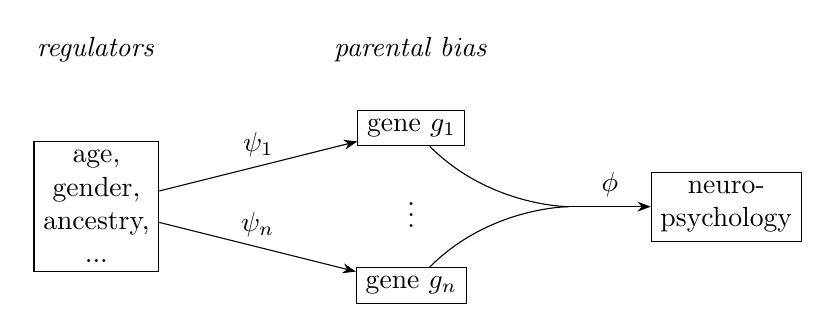
\begin{tikzpicture}[align=center]
\node at (-4,2) {\emph{regulators}};
\node[draw] (A) at (-4,0) {age,\\gender,\\ancestry,\\...};
\node at (0,2) {\emph{parental bias}};
\node[draw] (G1) at (0,1) {gene \(g_1\)};
\node at (0,0) {\vdots};
\node[draw] (Gn) at (0,-1) {gene \(g_n\)};
\coordinate (C) at (2,0);
\node[draw] (B) at (4,0) {neuro-\\psychology};
\draw[-Stealth] (A) -- node[anchor=south] {\(\psi_1\)} (G1);
\draw[-Stealth] (A) -- node[anchor=south] {\(\psi_n\)} (Gn);
\draw[-Stealth] (C) -- node[anchor=south] {\(\phi\)} (B);
\draw (G1) .. controls (1,0) and (2,0) .. (C);
\draw (Gn) .. controls (1,0) and (2,0) .. (C);
\end{tikzpicture}
\end{center}
\caption{}
\label{fig:scheme}
\end{figure}

Our genome-wide analysis suggests that \(<1\%\) of all genes are imprinted,
which implies \(n\approx 200\).  This provides evidence, in addition to
previous similarly conservative estimates of \(n\)
\cite{Perez2015,DeVeale2012}, against the controversial estimate of \(n\approx
1300\) \cite{Gregg2010a}.

More interestingly, we find that several regression coefficients differ
significantly from zero, which suggests that age, gender and ancestry do
indeed regulate parental bias in at least some imprinted genes in the human
DLPFC.  We infer that these three regulators exert gene-specific effects, up-
or down-regulating parental bias in a subset of imprinted genes while having
no (detectable) impact on the rest.  That these predictors differ in the
subset of genes they affect significantly hints at the potential complexity of
regulation.  A further layer of that complexity arises from possible
interactions among these predictors, which is in fact consistent with the
dependence of the age effect on gender in our conditional analysis.

The interpretation of the present results as the effect of (human) ancestry on
parental bias points to genetic regulatory mechanisms of imprinting that
modulate the known epigenetic mechanisms.  Given the late emergence of
imprinting in therian phylogeny and its role in neuropsychological and social
function, the genetics of parental bias may well be an increasingly important
target of natural selection.  Also, the ancestry effect is a remarkable
novelty of our work since previous studies, all using in-bread mouse strains,
failed to address this point.  As for age, a similar differential effect was
found in the mouse cerebellum to the effect we observe here. Gender, however,
had no significant effect in the same mouse study.

The above interpretation certainly depends on our statistical inference, which
in turn is based on the present data and regression models, both of which have
serious limitations.  Some of these---related to differing sequencing and
genotyping protocols---might be alleviated by improved across-institute
standardization.  But others, such as the confounding of age by certain
technical variables (e.g.~institution), are hopelessly entangled with the
observational nature of post mortem human studies, which precludes orthogonal,
that is clearly interpretable, decomposition of the variation of the observed
measure of parental bias (the response) into separate technical and biological
components.  In addition, non-orthogonality also limits statistical power.  But even
if the data fulfilled orthogonality, the present regression models would still
remain too rigid to account for the relative overdispersion of RNA-seq read
counts, the uncertainty surrounding haplotype, and that genes are neither
completely independent nor completely identical in their parental bias.  In
future work these ought to be tackled either with recently developed
hierarchical models built on normal linear model \cite{Perez2015,Law2014} or,
if regulators indeed strongly interact as the present work indicates, by the
adoption of Bayesian networks.

The molecular mechanism mediating the age effect.  TODO: clusters and regression
coefficients for gender and ancestry

Even if the regulatory effect of age, gender, ancestry, etc, on parental bias
is more firmly established by methodological improvements and more data, it
still remains to be determined whether (and how) the corresponding changes in
expression phenotype affect neural and psychological properties and might be
causal to some common psychiatric disorders.  This work may be considered an
initial step towards that aim as the estimated regression coefficients,
associated with SCZ or AFF, provide statistically weak hints at that
causality.

A more general question is how function \(\phi\) in Fig.~\ref{fig:scheme}
integrates parental bias across genes and maps that signal to organismal
phenotype.  That mapping occurs through the intermediate domain of cellular
metabolism.  Therefore, extending the present ``multi-omic'' data collection
with a metabolic layer appears promising, especially because rather specific
metabolism characterizes several imprinted genes \cite{Tucci2016,Peters2014}.
Adopting single-cell RNA-seq in the present framework would be another
interesting extension that could possibly elucidate the role of random
monoallelic expression.

In fact, the question regarding the map \(\phi\) is even more general, since
it is plausible that parental bias acts jointly with overall expression level
(this is not indicated in Fig.~\ref{fig:scheme}).  If so, the resolution of
the prevailing system biology is to be refined from mere genes to separate
maternal and paternal copies.  On the other hand, the present finding that
parental bias substantially varies across individuals even withing the same
tissue calls for a conceptual shift from the current practice of regarding
genes unconditionally as either imprinted or not to considering instead the
conditional distribution of their parental bias within the population given
regulators such as age, gender, and ancestry.

\bibliography{monoall-ms}

\section{Supplementary Material}

\newpage

% Supplementary figures

\setcounter{figure}{0}
\makeatletter 
\renewcommand{\thefigure}{S\@arabic\c@figure}
\makeatother

\begin{figure}
\begin{center}
\includegraphics{figures/by-me/monoall-M1}
\hspace{\fill}
\includegraphics{figures/by-me/monoall-M2}
\end{center}
\caption{AGK models: M1 (left) and M2 (right)}
\label{fig:agk}
\end{figure}

\begin{figure}
\begin{center}
\includegraphics[scale=0.6]{figures/2016-08-08-imprinted-gene-clusters/score-genomic-location-1.png}
\end{center}
\caption{}
\label{fig:clusters}
\end{figure}

\begin{figure}
\begin{center}
\includegraphics[scale=0.6]{figures/2016-08-01-ifats-filters/known-genes-1.pdf}
\caption{}
\label{fig:known-genes}
\end{center}
\end{figure}

\begin{figure}
\begin{center}
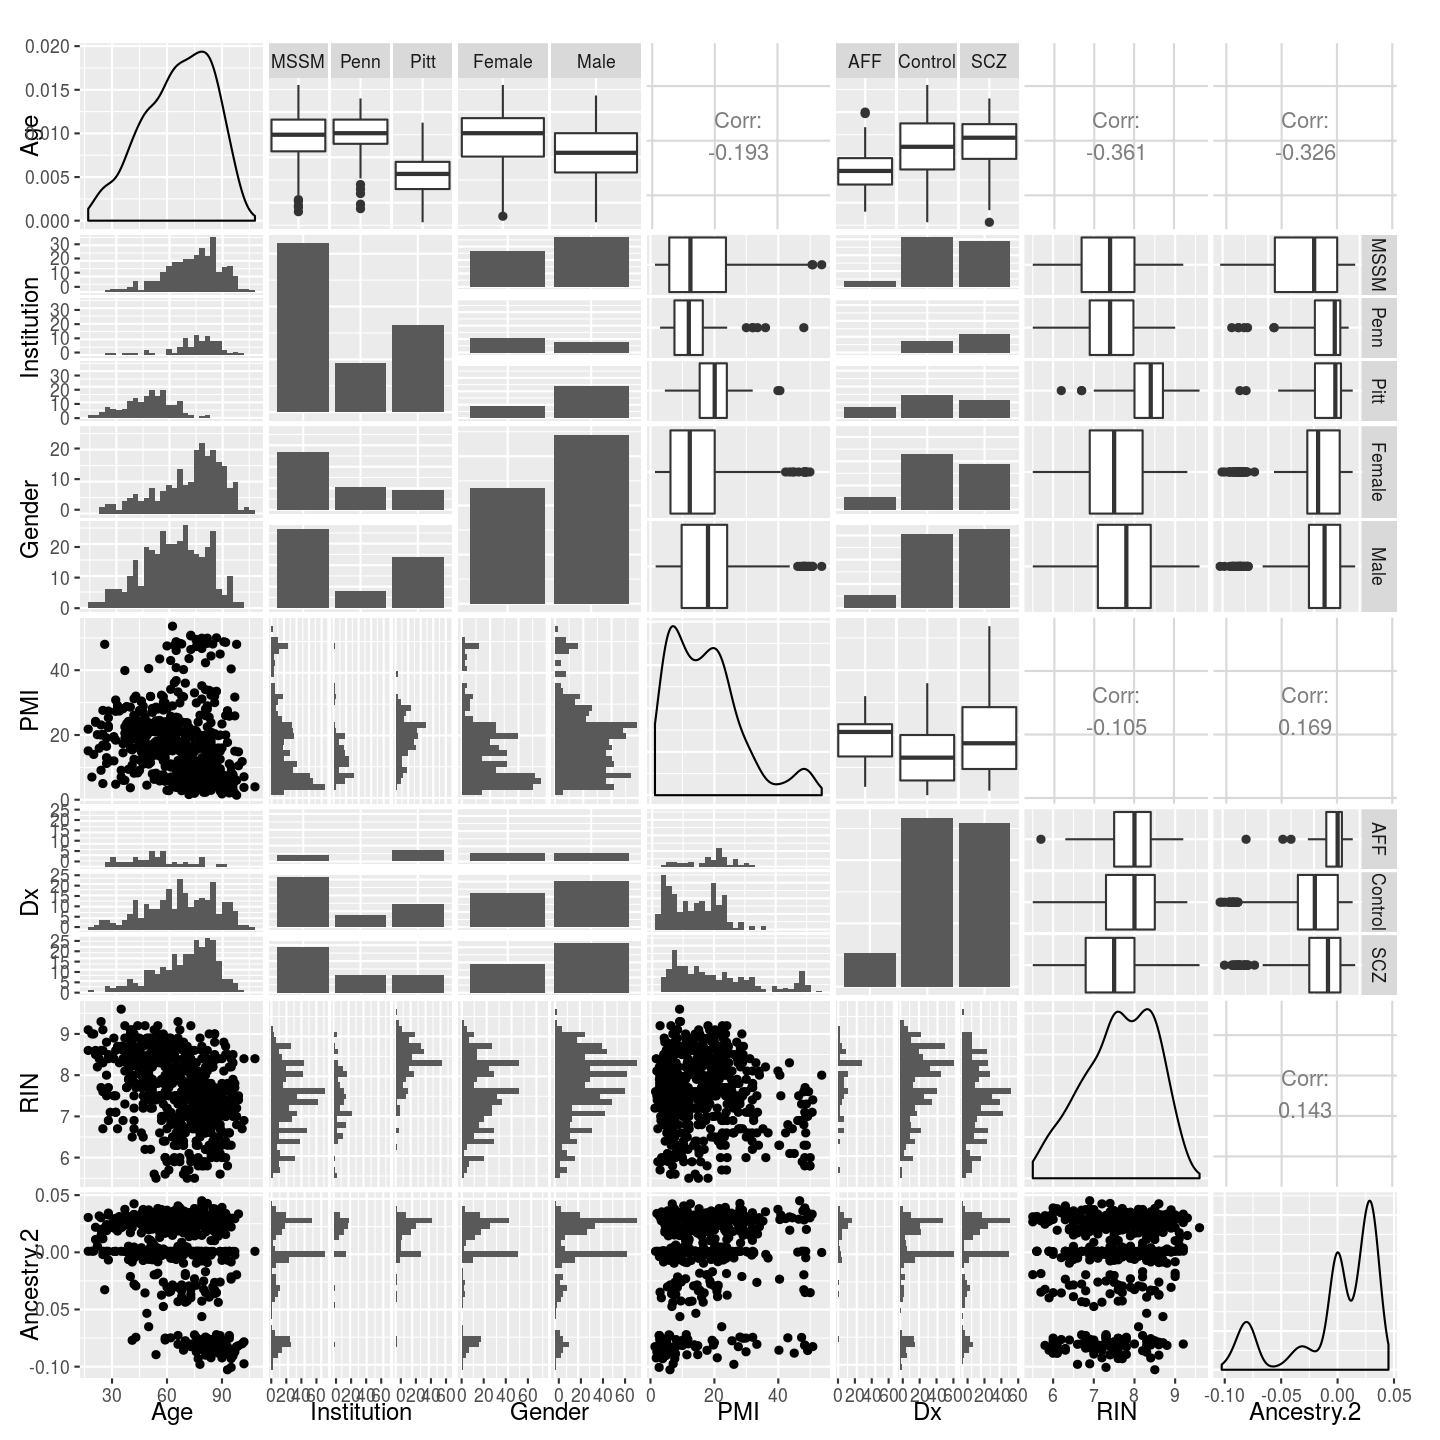
\includegraphics[scale=0.6]{figures/2016-06-26-trellis-display-of-data/evar-scatterplot-matrix-2.png}
\end{center}
\caption{}
\label{fig:predictor-associations}
\end{figure}

\begin{figure}
\begin{center}
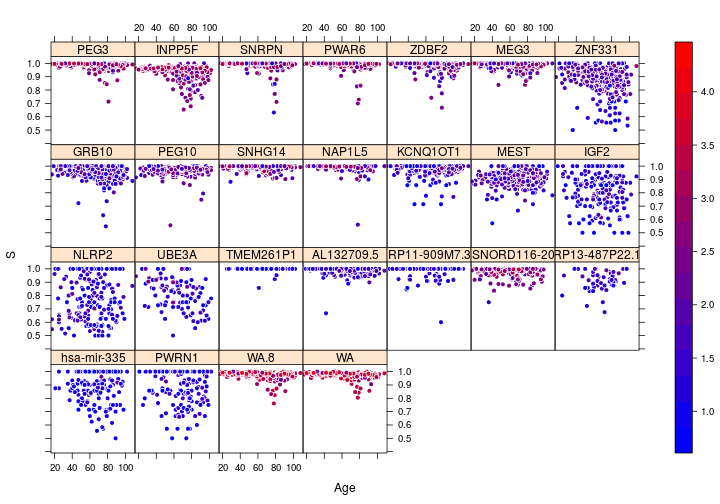
\includegraphics[scale=0.6]{figures/2016-06-26-trellis-display-of-data/S-age-tot-read-count-1.png}
\end{center}
\caption{}
\label{fig:weight-of-evidence}
\end{figure}

\begin{figure}
\begin{center}
\includegraphics[scale=0.6]{figures/2016-09-23-model-checking/qqnorm-wnlm-Q-1.pdf}
\end{center}
\caption{}
\label{fig:qqnorm-wnlm.Q}
\end{figure}

\begin{figure}
\begin{center}
\includegraphics[scale=0.6]{figures/2016-09-23-model-checking/qqnorm-logi-S-1.pdf}
\end{center}
\caption{}
\label{fig:qqnorm-logi.S}
\end{figure}

\begin{figure}
\begin{center}
\includegraphics[scale=0.6]{figures/2016-09-23-model-checking/homoscedas-wnlm-Q-1.pdf}
\end{center}
\caption{}
\label{fig:homoscedas-wnlm.Q}
\end{figure}

\begin{figure}
\begin{center}
\includegraphics[scale=0.6]{figures/2016-09-23-model-checking/homoscedas-logi-S-1.pdf}
\end{center}
\caption{}
\label{fig:homoscedas-logi.S}
\end{figure}

\begin{figure}
\begin{center}
\includegraphics[scale=0.6]{figures/2016-09-23-model-checking/influence-wnlm-Q-1.pdf}
\end{center}
\caption{}
\label{fig:influence-wnlm.Q}
\end{figure}

\begin{figure}
\begin{center}
\includegraphics[scale=0.6]{figures/2016-09-23-model-checking/influence-logi-S-1.pdf}
\end{center}
\caption{}
\label{fig:influence-logi.S}
\end{figure}

\begin{figure}
\begin{center}
\includegraphics[scale=0.6]{figures/2016-10-03-permutation-test/p-val-tdist-vs-perm-filt-iso-1.pdf}
\end{center}
\caption{}
\label{fig:pval-tdist-vs-perm}
\end{figure}

\begin{figure}
\begin{center}
\includegraphics[scale=0.6]{figures/2016-10-03-permutation-test/p-values-1.pdf}
\end{center}
\caption{}
\label{fig:pval}
\end{figure}

\begin{figure}
\begin{center}
\includegraphics[scale=0.6]{figures/2016-08-21-likelihood-surface/explain-rll-wireframe-1.png}
\includegraphics[scale=0.6]{figures/2016-08-21-likelihood-surface/explain-rll-levelplot-B-1.png}
\end{center}
\caption{}
\label{fig:ll-surf-explain}
\end{figure}

\begin{figure}
\begin{center}
\includegraphics[scale=0.6]{figures/2016-06-22-extending-anova/logi-S-wnlm-Q-compare-1.pdf}
\end{center}
\caption{}
\label{fig:logi.S-wnlm.Q-compare}
\end{figure}

\begin{figure}
\begin{center}
\includegraphics[scale=0.6]{figures/2016-06-22-extending-anova/reg-coef-wnlm-Q-1.pdf}
\end{center}
\caption{}
\label{fig:all-effects-wnlm.Q}
\end{figure}

\begin{figure}
\begin{center}
\includegraphics[scale=0.6]{figures/2016-06-22-extending-anova/reg-coef-logi-S-filt-1.pdf}
\end{center}
\caption{}
\label{fig:all-effects-logi.S}
\end{figure}

\begin{figure}
\begin{center}
\includegraphics[scale=0.6]{figures/2016-08-08-imprinted-gene-clusters/segplot-logi-S-99conf-1.pdf}
\end{center}
\caption{Biological effects: estimates and $99\%$ confidence intervals under
the logi.S model}
\label{fig:biol-effects-logi.S}
\end{figure}

\begin{figure}
\begin{center}
\includegraphics[scale=0.6]{figures/2016-08-21-likelihood-surface/ll-surf-coefs-wnlm-Q-1.png}
\end{center}
\caption{}
\label{fig:likelihood-surface}
\end{figure}

\begin{figure}
\begin{center}
\includegraphics[scale=0.6]{figures/2016-07-08-conditional-inference/beta-age-cond-wnlm-Q-2-1.pdf}
\end{center}
\caption{}
\label{fig:interaction-wnlm.Q}
\end{figure}

\begin{figure}
\begin{center}
\includegraphics[scale=0.6]{figures/2016-07-08-conditional-inference/beta-age-cond-logi-S-2-skip-1.pdf}
\end{center}
\caption{}
\label{fig:interaction-logi.S}
\end{figure}

\begin{figure}
\begin{center}
\includegraphics[scale=0.6]{figures/2016-06-22-extending-anova/anova-effects-fw-rv-wnlm-Q-1.pdf}
\end{center}
\caption{}
\label{fig:anova}
\end{figure}

\begin{figure}
\begin{center}
\includegraphics[scale=0.6]{figures/2016-10-20-differential-expression-scz/venn-triple-1.pdf}
\end{center}
\caption{}
\label{fig:diff-exp-scz}
\end{figure}

\begin{figure}
\includegraphics[width=0.6\textwidth]{figures/2016-10-11-comparison-to-mouse-cerebellum/posterior-pp-vs-pval-wnlm-Q-1.pdf}
\caption{Comparison of the effects of age and gender between the present work and a
previous study~\cite{Perez2015} in the mouse cerebellum. }
\label{fig:mouse-cerebellum}
\end{figure}

% Supplementary tables

\setcounter{table}{0}
\makeatletter 
\renewcommand{\thetable}{S\@arabic\c@table}
\makeatother

\end{document}
